\documentclass[conference]{IEEEtran}
\usepackage[utf8]{inputenc} 
\usepackage[T1]{fontenc}
\usepackage[english]{babel}
\usepackage{graphicx}
\usepackage{amssymb}
\usepackage{amsmath}
\usepackage{subcaption}
\usepackage{amsfonts}
\usepackage{makeidx}
\usepackage{multirow}
\usepackage{verbatim}
\usepackage[usenames]{color}
%\usepackage{algorithm}
%\usepackage{algorithmic}
\usepackage[]{algorithm2e}
\usepackage[noadjust]{cite}
\usepackage{mathtools}
\DeclarePairedDelimiter{\ceil}{\lceil}{\rceil}
\hyphenation{op-tical net-works semi-conduc-tor}
\usepackage{array}
\usepackage{tabularx}

\usepackage{pgfplots}
\pgfplotsset{width=10cm,compat=1.9}
\usepgfplotslibrary{external}
\usepackage{hyperref}
\providecommand{\keywords}[1]{\textbf{\textit{Keywords---#1}}}
\newcolumntype{P}[1]{>{\centering\arraybackslash}m{#1}}



\begin{document}
	\title{Image classification \\ with Feed-Forward Neural Networks}
	
	\author{\IEEEauthorblockN{Bartłomiej Meller \\ bartmel655@student.polsl.pl \\ Silesian University of Technology \\ Faculty of Mathematics \\ Kaszubska 23 \\ Gliwice 44-100 \and Kamil Matula \\ kamimat133@student.polsl.pl \\ Silesian University of Technology \\ Faculty of Mathematics \\ Kaszubska 23 \\ Gliwice 44-100 \and Paweł Chłąd \\ pawechl893@student.polsl.pl \\ Silesian University of Technology \\ Faculty of Mathematics \\ Kaszubska 23 \\ Gliwice 44-100}}

   

	
	\maketitle
	
	
	\begin{abstract}
	%streszczenie, 150--200 słów
	
	Artificial neural networks, such as feed-forward networks (FFN), convolutional neural networks (CNN), recursive neural network (RNN) are becoming powerful tools that are starting to replace many classical algorithms. It is known that, for image recognition, CNNs are often the best choice in terms of accuracy. In this paper we show that feed forward networks are capable of achieving comparable performance, with less complicated architecture in comparison to CNNs. After presentation of underlying theory of Feed Forward networks, we present different methods, that allowed us to get past network local minima, then we show experiments and conclusions that followed.
	
	
	\end{abstract}
	
	\vspace{5pt}
	\keywords{neural networks, activation function, images, classification}
	
	%\IEEEpeerreviewmaketitle
	
	\vspace{10pt}
	
	\section{Introduction}
	%Artykuł powinien być napisany w języku angielskim i zajmować około 6-7 stron.
	Artificial neural networks such as feed-forward networks (FFN), convolutional neural networks (CNN), recursive neural network (RNN) are becoming powerful tools that are starting to replace many classical algorithms. It is known that, for image recognition, CNNs are often the best choice in terms of accuracy. We went with FFN because they are simpler in their structure and with sufficient amount of data and heuristic approach they can achieve comparable performance, while being easier to implement and manage.
	
	One of the most effective learning method is backpropagation (BP) algorithm. BP uses gradient calculation to determine ''direction'' in which network should ''go''. The downside of strict mathematical approach is that gradient-based methods often ''get stuck'' in local minima of a function. Another common problem in many kinds of networks is knowledge generalization; we often train our models on large data sets, to avoid fixation of a network on small set of examples. This paper addresses both of those issues. We show that combining heuristic and backpropagation algorithm allows, for efficient overcoming of ''minima traps'' and methods that help networks to generalize their knowledge. First we introduce basic theory of Feed-Forward Networks, alongside with explanation of backpropagation algorithm. Then we describe our example model and series of experiments that were performed on the model. At the end of our paper, we present conclusion that we have gathered and give performance metrics of our model.
	
	
	\section{Feed-Forward Networks Theory}
	Artificial Neural Network (ANN) is a mathematical model of biological neural networks that compose a human brain; similarly to one, the ANN is built of neurons which are parts of layers. Each neuron from each layer is connected to all neurons from the previous layer and all neurons of the next layer are connected by synapses. These connections have randomly initialized weights, which are being modified in the learning process.
	
	The first layer, responsible for receiving input data, is called input layer. Similarly the last one, which returns output data, is called output layer. There can be zero, one or more hidden layers between them. The goal of neural network architect is to find optimal sizes of layers, to make learning process much more efficient. Input neurons' count depends on number of features the analyzing object has and output neurons' count on how many classes it can be classified to.
	
	Every neuron receives value on input, transforms it using activation function and sends the output signal to the next layer. The input signal of $i^{th}$ neuron of $k^{th}$ layer is:
	
	\begin{equation*}
	    s^k_i = \sum_{j=1}^{n}w^k_{ij} y^{k-1}_{j},
	\end{equation*}
	
	\noindent where $w^k_{ij}$ is a weight of connection between $i^{th}$ neuron of $k^{th}$ layer and $j^{th}$ neuron of previous layer and $y^{k-1}_{j}$ is $j^{th}$ neuron of previous layer's output signal value. The output signal of $i^{th}$ neuron is:
	
	\begin{equation*}
	    y^k_i = f(s^k_i) = f(\sum_{j=1}^{n}w^k_{ij} y^{k-1}_{j}).
	\end{equation*}
	
	\vspace{5pt}
	There are many activation functions (also known as transfer functions or threshold functions). One of the most commonly used is bipolar linear function. It's equation is:
	
	\begin{equation*}
	    f(s^k_i) = \frac{2}{1 + e^{-\alpha s^k_i}} - 1 = \frac{1 - e^{-\alpha s^k_i}}{1 + e^{-\alpha s^k_i}}
	\end{equation*}

	\vspace{5pt}
	\noindent where $\alpha$ is a coefficient that influences ''width'' (convergence rate) of activation function.  
	
\vspace{20pt}	
\begin{center}
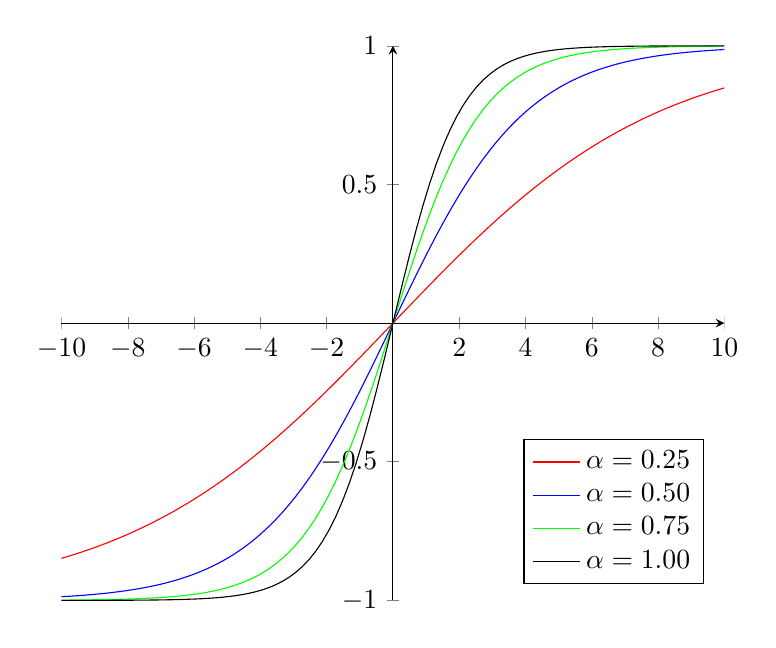
\begin{tikzpicture}
\begin{axis}[
    axis lines = middle,
    xmin = -10, xmax = 10,
    ymin = -1, ymax = 1,
    legend pos=south east
]

\addplot [
    domain=-10:10,
    samples=100, 
    color=red,
]
{(1 - exp(-0.25 * x))/(1 + exp(-0.25 * x))};
\addlegendentry{$\alpha = 0.25$}

\addplot [
    domain=-10:10,
    samples=100, 
    color=blue,
    ]
    {(1 - exp(-0.5 * x))/(1 + exp(-0.5 * x))};
\addlegendentry{$\alpha = 0.50$}

\addplot [
    domain=-10:10,
    samples=100, 
    color=green,
    ]
    {(1 - exp(-0.75 * x))/(1 + exp(-0.75 * x))};
\addlegendentry{$\alpha = 0.75$}

\addplot [
    domain=-10:10,
    samples=100, 
    color=black,
    ]
    {(1 - exp(-x))/(1 + exp(- x))};
\addlegendentry{$\alpha = 1.00$}

\end{axis}
\end{tikzpicture}
\newline Bipolar linear activation function
\end{center}
\vspace{20pt}

After artificial neural network has been properly built, it is time to teach it object recognition. ANN learns by adjusting synaptic weights in strictly defined way. There are many methods of learning, but the most popular training technique that is used in Feed-forward Neural Network is back-propagation in which modifying weights of the connections goes from output layer to input layer sequentially. This direction is opposite to the way inserted information moves in all FFNs. The goal of training process is to minimize the value of loss function, for all elements included in training set (T). The training set consists of input vectors, which are inserted to first layer by input synapses, and expected output vectors, which are compared with gained outputs every time neural network is fed. The loss function shows the distance between predicted value and the actual one. To calculate it we can use Mean Square Error Loss or Cross-Entropy Loss (also known as Log Loss). Using MSE, total error of training set can be described with equation:

    \begin{equation*}
        E = \sum_{T}\sum_{i=1}^{n}(d_{i} - y_{i})^{2},
    \end{equation*}

\vspace{5pt}    
\noindent where $n$ is a dimension of output vector (and also count of neurons on output layer), $d_i$ is predicted value on $i^{th}$ position of output vector and $y_i$ is actual value on $i^{th}$ position of output vector. Correction of synaptic weights starts in last layer and goes backwards through all hidden layers until it reaches input layer. The weight is changed according to equation:

    \begin{equation*}
        w^k_{ij} = w^k_{ij} + \eta \nabla w^k_{ij},
    \end{equation*}

\vspace{5pt}    
\noindent where $\eta$ is correcting coefficient commonly called 'Learning Rate' and $\nabla w^k_{ij}$ is a value of gradient of synapse's weight's error:

    \begin{equation*}
        \nabla w^k_{ij} = \frac{\partial E}{\partial w^k_{ij}} = \frac{1}{2} \cdot \frac{\partial E}{\partial s^k_i} \cdot 2 \cdot \frac{\partial s^k_i}{\partial w^k_{ij}} = 2 \delta^k_i y^{k-1}_j,
    \end{equation*}
    
\vspace{5pt}
\noindent where $\delta^k_i$ is value of a change of error function, for $k^{th}$ layer's $i^{th}$ neuron's input signal and $y^{k-1}_j$ is previous layer's $j^{th}$ neuron's output signal value. On last, $K^{th}$ layer $\delta$ equals:

    \begin{equation*}
        \delta^K_i = \frac{1}{2} \cdot \frac{\partial E}{\partial s^k_i} = \frac{1}{2} \cdot \frac{\partial (d^K_{i} - y^K_{i})^2}{\partial s^k_i} = f'(s^K_i) \cdot (d^K_{i} - y^K_{i}),
    \end{equation*}
 
 \vspace{5pt}   
\noindent where $f'(s^K_i)$ is value of activation function's differential of $i^{th}$ output neuron's input signal. On this layer the value depends mainly on distance between predicted and actual values - on error. Other layers' $\delta$s use numbers calculated in previous steps:

    \begin{equation*}
        \delta^k_i = \frac{1}{2} \cdot \frac{\partial E}{\partial s^k_i} = \frac{1}{2} \cdot \sum_{j=1}^{N_{k+1}} \frac{\partial E}{\partial s_j^{k+1}} \frac{\partial s_j^{k+1}}{\partial s^k_i} = f'(s^k_i) \sum_{j=1}^{N_{k+1}} \delta^{k+1}_j w^{k+1}_{ij},
    \end{equation*}
 
\vspace{5pt}   
\noindent where $N_{k+1}$ is count of neurons on $(k+1)^{th}$ layer.

\vspace{15pt}
In Algorithm 1 you can see the full process of training Feed-Forward Neural Network using back-propagation algorithm. It uses array called $D$, which consists of $\delta$ values. This jagged array has $L$ rows and as many columns, in a row, as many neurons the layer has, it corresponds to. All elements of arrays are written like $A_{i,j}$ which is just alternative form, for writing $A[i][j]$. What's more, numerical intervals that are used in the for-loops are half-open (the numbers after \textbf{to} don't count to these intervals). There are also symbols like $LR$, $s^k_i$, $y^k_i$ and $w^{k}_{ij}$. They mean respectively: Learning Rate ($\eta$), $k^{th}$ layer's $i^{th}$ neuron's input and output values and weight of synapse between $i^{th}$ neuron of $k^{th}$ layer and $j^{th}$ neuron of previous layer. Moreover there is $f'(\cdot)$ symbol that signifies the differential of the activation function - for bipolar linear function 
\vspace{5pt}
\begin{equation*}
   f(x) = \frac{1 - e^{-\alpha x}}{1 + e^{-\alpha x}} 
\end{equation*}

\vspace{5pt}
\noindent the differential is:
\vspace{5pt}
\begin{equation*}
f'(x) = \frac{2 \alpha e^{-\alpha x}}{(1 + e^{-\alpha x})^2}.    
\end{equation*}

\newpage

\begin{algorithm}
\vspace{50pt}
\KwData{$EpochsCount$, $TrainingInputs$, $ExpectedOutputs\ (EOUT)$}
\KwResult{Higher precision of neural network}
$L := $ count of network's layers\;
$D := $ empty jagged array, for $\delta$\ values\;
\For{$i = 0$ \KwTo $EpochsCount$}{
\For{$j = 0$ \KwTo Training Set's Length}{
Insert $j^{th}$ vector from $Inputs$ \\ to first layer's input synapses\;
\vspace{5pt}
\For{$k = 0$ \KwTo L}{
Calculate $s^k$ on all neurons on $k^{th}$ layer \\ by summing products of synaptic weights \\ and output values of previous layer \\ neurons (or synapses if it is input layer)\;
\vspace{5pt}
Calculate $y^k$ on all neurons on $k^{th}$ layer \\ by using activation function\;
}
\vspace{5pt}
$Output\ (OUT) := $ vector made of output values\\ values from output neurons\; 
\For{$n = 0$ \KwTo output neurons count}{
$D_{(L-1),n} = (EOUT_{j,n} - OUT_j) \cdot f'(s^{L-1}_n)$\;
}
\vspace{5pt}
\For{$k = L-2$ \KwTo $0$ \textbf{step} $-1$}{
\For{$n = 0$ \KwTo $k^{th}$ layer's neurons count}{
$D_{k,n} = 0$\;
\For{$m = 0$ \KwTo $(k+1)^{th}$ layer's \\ neurons count}{
$D_{k,n} = D_{k,n} + D_{(k+1),m} \cdot w^{k+1}_{mn}$\;
}
$D_{k,n} = D_{k,n} \cdot f'(s^{k}_n)$\;
}
}
\vspace{5pt}
\For{$k = L-2$ \KwTo $0$ \textbf{step} $-1$}{
\For{$n = 0$ \KwTo $k^{th}$ layer's neurons count}{
\For{$m = 0$ \KwTo $(k-1)^{th}$ layer's \\ neurons count}{
$w^{k}_{nm} = 2 \cdot LR \cdot D_{k,n} \cdot y_m^{k-1}$\;
}
}
}
}        
}
\caption{FFN training algorithm.}
\end{algorithm}

\vspace{50pt}
	\section{Example system}
	Our experimental FFN takes in an 50x25x3 image and outputs six dimensional vector of decision values. Each decision value represents one movie that is associated with given frame.
	\subsection{Data preparation}
	\subsubsection{Image preparation} After loading data set into the memory, we cut each image to meet 2:1 aspect ratio, this value was chosen because our input vector is an image that has an aspect ratio 2:1. If we took an image with aspect ratio that does not meet input aspect ratio, we would need to stretch or shrink an image; that would in turn add some pixels and thus make results more inaccurate. After cropping to target aspect ratio, we crop another $\frac{1}{12}$ of width and height, from each side, to eliminate possible letterboxes. Finally we shrink an image to get it to 50x25 dimensions. Such dimensions have been chosen to cut down on training times.
	\subsubsection{Data labeling}
	Each image is given label, signifying movie it belongs to. Then $\frac{1}{10}$ of image samples are redirected into testing set.
	\subsection{Training network}
	After preparation of training and testing datasets, all 225 per movie images, converted to the vectors, are inserted to the neural network. As it was said in ''Feed-Forward Networks Theory'' section, the information goes through all layers to the output layer with using activation function in all encountered neurons and then goes back in back-propagation process, modifying synaptic weights. This sequence is repeated multiple times and results in improvement of network's ability to recognizing objects.

\section{Experiments}
	Main problem that was dealt with in order to provide optimal learning accuracy and time, was selecting appropriate architecture that grants relatively good accuracy, but on the other hand, contains as few neurons as required. Minimal neuron count results in minimal computational time.
	
	Initially, when tests were carried out on 4 classes of data, network that contained only one hidden layer which consisted of as few as 50 neurons seemed to be the most efficient and accurate (76\%). Nevertheless it was not capacious enough to accommodate amount of knowledge that could recognize four or more movies. Eventually, model that contained 3 hidden layers with the following count of neurons: 800, 200, 50 came out to be an optimal solution.
	
	The back-propagation algorithm has one significant defect. It does not use any heuristics that could help it to deal with local minima. Solution to this issue is quite simple and easy to implement. In this case, adding a random number from range of $[-0.002;0.002]$ to weights of all connections turned out to be extraordinarily efficient. However it's hard to say about exact values because, the method was crossed with gradual increase of classes count.
	
	Surprisingly, increasing amount of classes resulted in leap of quality in decisions made by the network. This phenomenon was observed, after few epochs of learning, after class addition. Sometimes network needed randomization mentioned above for the phenomenon to occur.
	
	At the time of writing this article absolute accuracy of predictions made by the network, for six classes exceeded maximal accuracy given on four classes. We suspect that this could be explained by growing generality of classifier contained in the model with increasing amount of known classes.
        
    Methodology of learning was following. Model was trained until it's accuracy hadn't increased, for few epochs. In next stage networks' weights was randomized to get three different child networks. All four instances was learned in parallel. At the end, the best one of them was picked, reproduced by randomizing their weights and then all the process were repeated. When the network had stalled with it's advancement, one class was added to its possible outputs and learning was continued in the same way.
    
    One of the most interesting issues that we have experienced in the initial part of the research was a significant drop in accuracy when class set contained ''Shrek 2'' movie. After preliminary learning on dataset that hadn't contained this movie, this problem disappeared.
    
    We were also experimenting with different weight initialization techniques, described in \cite{WeightInit}. We have tried the following methods:
    \begin{itemize}
        \item He weight initialization - multiplies random value $[-1.0, 1.0]$ with $\sqrt{\frac{2}{size}}$ where $size$ is a size of previous layer
        \item Xavier's weight initialization - similar to He initialization, but with $\sqrt{\frac{1}{size}}$
        \item We also used the following technique: $\sqrt{\frac{2}{size_{l-1} + size_{l}}}$ where $size_n$ is size of nth layer
    \end{itemize}
    
    Unfortunately none of those methods worked correctly. In testing, we used networks with significant number of neurons in nearly every layer (3750 neurons in input layer) that in turn set initial weight values to minute values.
    

\vspace{5pt}
    Results of our research are shown in the tables below.
\vspace{5pt}
    
\begin{center}
\begin{tabular}{|| c | c ||} 
\hline
\multicolumn{2}{||c||}{1 hidden layer with 50 neurons} \\
 \hline
 Movies count & Highest precision \\
 \hline
 4 & 76.0 \% \\
 \hline
 5 & 71.2 \% \\ 
 \hline
 6 & 52.7 \% \\ 
 \hline
\end{tabular}
\end{center}

\vspace{5pt}
\begin{center}
\begin{tabular}{|| c | c ||} 
\hline
\multicolumn{2}{||c||}{3 hidden layers: 800, 200 and 50 neurons} \\
 \hline
 Movies count & Highest precision \\
 \hline
 4 & 82.0 \% \\
 \hline
 5 & 88.8 \% \\ 
 \hline
 6 & 84.6 \% \\ 
 \hline
\end{tabular}
\end{center}

\vspace{5pt}
First table presents the most satisfactory accuracies of the neural network (with 1 hidden layer consisting of 50 neurons) before the experiment. The second one shows the effects of randomization. Percents situated in right columns are calculated by dividing amount of correctly recognized movies by size of testing dataset (which is 25 frames per movie). As it shows, the results are surprisingly high.

\vspace{10pt} 
	\section{Example Predictions}

The tables below contain example predictions made by the network. Provided images are screenshots from the Netflix platform that were taken independently from the learning and testing datasets.

\vspace{5pt} 
\begin{table}[ht]
  \begin{tabular}{||P{2cm}|P{1.0cm}|P{1.2cm}|P{1.0cm}|P{1.2cm}||}

  \hline Picture & Origin & Prediction & Matches & 2nd prediction\\
  \hline\vspace{0.1cm}
  \includegraphics[width=2cm]{indiana_0.png} & Indiana Jones & Indiana Jones & \textbf{yes} & Shark Tale\\
  
  \hline\vspace{0.1cm}
  \includegraphics[width=2cm]{indiana_1.png} & Indiana Jones & Indiana Jones & \textbf{yes} & Shrek 2\\
  
  \hline\vspace{0.1cm}
  \includegraphics[width=2cm]{indiana_2.png} & Indiana Jones & Indiana Jones & \textbf{yes} & Shrek 2\\
  
  \hline\vspace{0.1cm}
  \includegraphics[width=2cm]{indiana_3.png} & Indiana Jones & Shrek 2 & no & The Lego Movie\\
  
  
  \hline\vspace{0.1cm}
  \includegraphics[width=2cm]{lego_0.png} & The Lego Movie & The Lego Movie & \textbf{yes} & Shark Tale\\
  
  \hline\vspace{0.1cm}
  \includegraphics[width=2cm]{lego_1.png} & The Lego Movie & The Lego Movie & \textbf{yes} & Shark Tale\\
  
  \hline\vspace{0.1cm}
  \includegraphics[width=2cm]{lego_2.png} & The Lego Movie & Shark Tale & no & The Lego Movie\\
  
  \hline\vspace{0.1cm}
  \includegraphics[width=2cm]{lego_3.png} & The Lego Movie & The Lego Movie & \textbf{yes} & Shrek 2\\
  
  
  
  
  \hline\vspace{0.1cm}
  \includegraphics[width=2cm]{madagascar_0.png} & Mada- gascar & Mada- gascar & \textbf{yes} & Shark Tale\\
  \hline\vspace{0.1cm}
  \includegraphics[width=2cm]{madagascar_1.png} & Mada- gascar & Shrek 2 & no & The Lego Movie\\
  \hline\vspace{0.1cm}
  \includegraphics[width=2cm]{madagascar_2.png} & Mada- gascar & Mada- gascar & \textbf{yes} & Shrek 2\\
  \hline\vspace{0.1cm}
  \includegraphics[width=2cm]{madagascar_3.jpg} & Mada- gascar & Mada- gascar & \textbf{yes} & Shrek 2\\
  
  

  \hline
  \end{tabular}
\end{table}
	
\newpage	
\vspace{5pt} 
\begin{table}[ht]
  \begin{tabular}{||P{2cm}|P{1.0cm}|P{1.2cm}|P{1.0cm}|P{1.2cm}||}

  \hline Picture & Origin & Prediction & Matches & 2nd prediction\\
\hline\vspace{0.1cm}
  \includegraphics[width=2cm]{sharktale_0.png} & Shark Tale & Shark Tale & \textbf{yes} & The Lego Movie\\
  
  \hline\vspace{0.1cm}
  \includegraphics[width=2cm]{sharktale_1.png} & Shark Tale & Shark Tale & \textbf{yes} & Indiana Jones\\
  
  \hline\vspace{0.1cm}
  \includegraphics[width=2cm]{sharktale_2.png} & Shark Tale & Shark Tale & \textbf{yes} & The Lego Movie\\
  
  \hline\vspace{0.1cm}
  \includegraphics[width=2cm]{sharktale_3.png} & Shark Tale & Shark Tale & \textbf{yes} & The Lego Movie\\
  
  

  
  \hline\vspace{0.1cm}
  \includegraphics[width=2cm]{shrek2_0.jpg} & Shrek 2 & Shrek 2 & \textbf{yes} & Shark Tale\\
  
  \hline\vspace{0.1cm}
  \includegraphics[width=2cm]{shrek2_1.jpg} & Shrek 2 & Shrek 2 & \textbf{yes} & Indiana Jones\\
  
  \hline\vspace{0.1cm}
  \includegraphics[width=2cm]{shrek2_2.jpg} & Shrek 2 & Shrek 2 & \textbf{yes} & Mada- gascar\\
  
  \hline\vspace{0.1cm}
  \includegraphics[width=2cm]{shrek2_3.jpg} & Shrek 2 & Shrek 2 & \textbf{yes} & Shark Tale\\
  
  
  
  
  \hline\vspace{0.1cm}
  \includegraphics[width=2cm]{vincent_0.png} & Loving Vincent & Loving Vincent & \textbf{yes} & Shrek 2\\
  
  \hline\vspace{0.1cm}
  \includegraphics[width=2cm]{vincent_1.png} & Loving Vincent & Loving Vincent & \textbf{yes} & The Lego Movie\\
  
  \hline\vspace{0.1cm}
  \includegraphics[width=2cm]{vincent_2.png} & Loving Vincent & Loving Vincent & \textbf{yes} & Shark Tale\\
  
  \hline\vspace{0.1cm}
  \includegraphics[width=2cm]{vincent_3.png} & Loving Vincent & Loving Vincent & \textbf{yes} & Shrek 2\\

  \hline
  \end{tabular}
\end{table}

As it can be seen, the accuracy is satisfactory high. It makes a few mistakes when it comes to dark and distant frames. Fixing this issue will be our next goal.

\vspace{5pt} 
	\section{Conclusions}
	After all experiments done with this network, we can state the following conclusions:
	\begin{enumerate}
	    \item \textit{Combining back-propagation and heuristic approach gave an unprecedented leap in network accuracy.} - After a number of tests with weight randomization, we suspect that by giving a ''nudge'' to weights, we push it out of local minimum, hence allowing it further learning.
	    \item \textit{Changing model in-flight allows, for more generality.} - By changing model topology (ex. adding additional output dimension), we have seen an increase in generality of a model.
	    \item \textit{Training on diversified samples first, results in increased generality.}
	\end{enumerate}
	
	We have shown that adding heuristics to strict algorithm of back-propagation helps in learning of neural networks. 

\vspace{10pt}
\begin{thebibliography}{9}
\bibitem{ffns} 
Information Resources Management Association, 
\textit{Deep Learning and Neural Networks: Concepts, Methodologies, Tools, and Applications}, \\ pp. 112-120, 2019, \url{https://books.google.pl/books?id=gsexDwAAQBAJ}.

\bibitem{loss functions} 
Jason Brownlee,
\textit{Loss and Loss Functions for Training Deep Learning Neural Networks}, 2019,
\url{https://machinelearningmastery.com/loss-and-loss-functions-for-training-deep-learning-neural-networks/}.
\bibitem{ffnt}
\textit{Michael A. Nielsen, "Neural Networks and Deep Learning", Determination Press, 2015}
\url{http://neuralnetworksanddeeplearning.com/}
\bibitem{WeightInit}
\href{https://towardsdatascience.com/weight-initialization-techniques-in-neural-networks-26c649eb3b78}{https://towardsdatascience.com/weight-initialization-techniques-in- \\ neural-networks-26c649eb3b78}
\end{thebibliography}

\end{document}